\documentclass{article}
\usepackage[UTF8]{ctex}
\usepackage{newtxtext}
\usepackage{geometry}
\usepackage[dvipsnames,svgnames]{xcolor}
\usepackage[strict]{changepage} % 提供一个 adjustwidth 环境
\usepackage{framed} % 实现方框效果
\usepackage{setspace}
\usepackage{tikz}
\usepackage{tcolorbox}
\usepackage{amsmath}
\usepackage{graphicx}
\usepackage{wrapfig}
\usepackage{float}

\geometry{a4paper,centering,scale=0.8,left=1.0cm,right=1.0cm,top=2.0cm,bottom=2.0cm}

\definecolor{blueshade}{rgb}{0.95,0.95,1} % 文%本框颜色
\definecolor{greenshade}{rgb}{0.90,0.99,0.91} % 绿色文本框,竖线颜色设为 Green
\definecolor{redshade}{rgb}{1.00,0.90,0.90}% 红色文本框,竖线颜色设为 LightCoral
\definecolor{brownshade}{rgb}{0.99,0.97,0.93} % 莫兰迪棕色,竖线颜色设为 BurlyWood
\definecolor{yellowshade}{rgb}{1,0.945,0.7255}%米黄色
\definecolor{DarkYellow}{rgb}{0.7843,0.61176,0.0549}

\newenvironment{formal}[2][greenshade]{%
\def\FrameCommand{%
\hspace{1pt}%
{\color{#2}\vrule width 2pt}%
{\color{#1}\vrule width 4pt}%
\colorbox{#1}%
}%
\MakeFramed{\advance\hsize-\width\FrameRestore}%
\noindent\hspace{-4.55pt}% disable indenting first paragraph
\begin{adjustwidth}{}{7pt}%
\vspace{2pt}\vspace{2pt}%
}
{
\vspace{2pt}\end{adjustwidth}\endMakeFramed%
}



\title{\Huge 金融市场学    \\\large made by  \LaTeX}
\author{NP\_123}


%\begin{tcolorbox}
%    [colback=Emerald!10,colframe=cyan!40!black,title=\textbf{公式}]
%\end{tcolorbox}

\begin{document} 
\begin{figure}[H]
    \begin{center}
        
\includegraphics[width=0.3\textwidth]{logo.jpeg}
        \maketitle
    \end{center}
\end{figure}
\thispagestyle{empty}
\clearpage
\section*{\center\Huge 资本市场-股票市场}
\subsection*{概念和种类}
\begin{itemize}
    \item 可以分为一级市场、二级市场。
    \item 股票是投资者向公司提供资本的权益合同,是所有权凭证。
    \item 股东拥有剩余索取权、剩余控制权、有限责任制。
    \item 股票本身没价值,但代表取得一定收入的权利,转让时不直接影响真实资本运动,一般不得退股。
\end{itemize}
\subsection*{普通股}
权利:享有剩余控制权,在优先股之后参与利益分配,上不封顶下不保底;
享有优先任股权(增发新股时按原持股比例购入股票的权利,该权利可出售)
\begin{itemize}
    \item 普通股A级可正常参与分红,但只有部分投票权(比如一股对1/3票)
    \item 普通股B级正常参与分红,享有完全投票权。常出现于老股东想集资但又不想过多放弃控制权。
    \item A股仅限中国内地居民以人民币购买。
    \item B股目前境内外投资者均可以外币购买。
\end{itemize}
普通股按风险特征分类
\begin{enumerate}
    \item 蓝筹股(大公司,稳定盈利,定期分红,公认投资价值高)
    \item 成长股(销售额利润迅速增长,且增速快于整个国家与其行业;低分红;高资本利得)
    \item 收入股/绩优股(当前能支付较高收益)
    \item 周期股(收益随经济周期波动)
    \item 防守股(面对不确定因素与经济衰退,收益率高于社会平均。比如公用事业)
    \item 概念股(依靠某一种题材支撑价格)
    \item 投机股(价格极不稳定或公司前景难以确定)
\end{enumerate}

\textbf{蓝筹股与成长股区别:
蓝筹股规模大,在行业内通常有较强的支配地位,绩优股业绩不错有一定规模
蓝筹股抗风险能力更强}
\subsection*{优先股}
权利:剩余索取权优先于普通股,分得固定利息,且在普通股前收取股息。
但一般没投票权,只有特殊投票权(比如无法按时支付优先股股息时,享有投票权到支付为止,
总而言之就是影响优先股股东投资利益)。

特点:由于收固定利息,优先股价格与经营状况联系不如普通股,风险小于普通股。
\begin{enumerate}
    \item 累积优先股
    \item 参加优先股(分为无限参加优先股和优先参加优先股)固定股息之后参加分配
    \item 可转换优先股(按比率转为普通股,常行使于普通股猛涨或意图加强公司控制)
    \item 可赎回优先股(允许公司按条件赎回)
\end{enumerate}

\subsection*{股票指数}
样本股票必须具有典型性和普遍性;计算方法要科学;基期的选择具有较好的均衡性和代表性;要排除非价格因素的影响。
\subsubsection*{股票价格平均数}
股票价格平均数反映一定时点上股票价格的绝对水平。没有基期的概念。
\begin{enumerate}
    \item 简单算数股权平均数(原道琼斯工业指数)\\
    优点:计算简单
    
    缺点:未考虑权重,未能区分重要性不同股票的不同影响;当有非价格因素影响时,失去连续性,使前后期比较困难
    \item 修正的股价平均数(基于简单算数股权平均数)
    分为:除数修正法和股价修正法

    除数修正法(如现道琼斯指数):修改除数

    股价修正法:假设J股票进行拆细,拆细前:股价P,拆细后:每股增加R股,股价为$P^*$。有$P=(1+R)P^*$。
    \item 加权股价平均数
    根据各个样本股的相对重要性加权。权数可以为成交股数、股票总市值$\ldots $
\end{enumerate}
\subsubsection*{股价指数}
股价指数是反映不同时点上股价变动情况的相对指标。常将报告期股价与选定基期比较。
\begin{enumerate}
    \item 简单算术股价指数(相对法,综合法)
    \item 加权股价指数(拉斯拜尔指数、派许指数):
    拉斯拜尔指数以基期作为权重,派许指数以报告期作为权重。绝大多数用派许指数。
\end{enumerate}



\clearpage
\section*{\center\Huge 货币市场}
\subsection*{同业拆借市场}
金融机构之间以货币借贷方式进行短期资金融通活动的市场。
\begin{itemize}
    \item 形成和发展\\
    产生于存款准备金政策的实施,伴随着中央银行业务和商业银行业务的发展而发展。
    拆借交易不仅发生在银行之间,还发生在银行与其它金融机构之间。
    \item 同业拆借市场的参与者\\
    商业银行、非银行金融机构、外国银行的代理机构和分支机构
    \item 运作程序:
    通过中介机构的同城拆借、通过中介结构进行的异地拆借、不通过中介机构的同城拆借、不通过中介机构的异地拆借
    \item 拆借期限与利率
    1—2天、隔夜、1—2周、1个月、接近或达到一年,按日计息
\end{itemize}
\subsection*{回购市场}
从本质上说,回购协议是一种抵押贷款,其抵押品为证券。
\begin{itemize}
    \item 交易原理:
    资金供应者、资金获得者,逆回购协议是从资金供应者的角度出发相当于回购协议而言的,是回购协议的逆进行。
    \item 回购市场及其风险\\
    {\color{red}{$\star$}}对于中央银行来说,通过回购交易可以实施公开市场操作,所以,回购市场是其执行货币政策的重要场所。
    \[I=PP\times RR\times T / 360  \hspace*{35pt} RP=PP+I\]
    (PP表示本金,RR表示证券商和投资者所达成的回购时应付的利率,T表示回购协议的期限,I表示应付利息,RP表示回购价格。)
    \item 利率的决定
    回购证券的质地、回购期限的长短、交割的条件、货币市场其它子市场的利率水平。\\
    {\color{red}{$\star$}}质押式回购利率比买断式回购利率低
\end{itemize}
\clearpage
\subsection*{商业票据市场}
商业票据是大公司为了筹措资金,以贴现方式出售给投资者的一种短期无担保承诺凭证。
\begin{itemize}
    \item 历史:
    \item 市场要素\\
    发行者:金融性和非金融性公司;面额大、期限短\\
    销售渠道:发行者通过自己的销售力量直接出售,通过商业票据交易商简介销售;信用评估\\
    {\color{red}{$\star$}}二级市场并不活跃,因为期限短,高度异质性\\
    发行价格和发行成本:
    \[\text{商业票据实际利率}=\frac{\text{折扣额}}{\text{发行价格}}\times \frac{360}{\text{距到期日天数}} \hspace*{35pt}  \text{折扣额}=\text{面额}-\text{发行价格}\]
    \[\text{发行价格}=\frac{\text{面额}}{1+\text{实际利率}\times \frac{\text{距到期日天数}}{360}}\]
    非利息成本:信用额度支持的费用,代理费用,信用评估费用;投资者
\end{itemize}

\subsection*{汇票市场}
分为商业承兑汇票与银行承兑汇票
\begin{itemize}
    \item 原理\\
    \textbf{银行承兑汇票的产生}:方便商业交易活动,在对外贸易中运用较多\\
    \textbf{在国际贸易中的优势}:1.出口商可以立刻获得货款进行生产
    2.避免了国际贸易中不同货币结算上的麻烦及利率风险
    3.银行做担保,无需调查信用状况\\
    \textbf{在国内贸易中的运用}:外汇承兑汇票
    \item 初级市场:出票,承兑(提示承兑、承兑、交还票据)
    \item 二级市场:背书、贴现、转贴现、再贴现
    \item 价值分析\\
    \textbf{借款人角度}:传统银行贷款的成本比运用银行承兑汇票的成本高,借款者用银行承兑汇票比发行商业票据筹资有利\\
    \textbf{从银行角度}:增加经营效益,增加其信用能力,银行出售银行承兑汇票不要求缴纳准备金\\
    \textbf{投资者角度}:收益性、安全性和流动性
\end{itemize}

\subsection*{大额可转让存单}
可以流通转让,金额大,比同期定期存款利率高,利率有固定的,也有浮动的
\begin{itemize}
    \item 种类:国内存单、欧洲美元存单、洋基存单、储蓄机构存单
    \item 风险:信用风险、市场风险
    \item 收益:发行银行的信用评级、存单的期限及存单的供求量
    \item 投资者:\textbf{大企业、金融机构}、政府机构、外国政府、外国中央银行、个人
    \item 价值分析\\
    \textbf{投资者角度}:较高利息收入、可随时获得兑现、收益稳定\\
    \textbf{银行角度}:增加资金来源、调整资产的流动性、实施资产负债管理 
\end{itemize}

\subsection*{短期政府债券市场}
一般来说,政府短期债券市场主要指的是国库券市场。
\begin{itemize}
    \item 发行方式:贴现方式,拍卖方式(竞争性方式、非竞争性方式)
    \item 发行目的:满足政府部门短期资金周转的需要,为中央银行的公开市场业务提供可操作的工具 
    \item 市场特征:违约风险小,流动性强,面额小,收入免税\\
    真实年收益率:所有资金按实际投资期所赚的相同收益率再投资的话,原有投资资金在一年内的增长率,考虑复利因素
    \begin{tcolorbox}
        [colback=Emerald!10,colframe=cyan!40!black,title=\textbf{计算}]
        \begin{align}
            \text{银行贴现收益率:}&\hspace*{20pt}Y_{BD} =\frac{F-P}{F}\times \frac{360}{t}\times 100\%  \hspace*{45pt} P=F\times (1-Y_{BD}\times \frac{t}{360})\nonumber\\
            \text{真实年收益率:}&\hspace*{20pt}Y_E ={(1+\frac{F-P}{P})}^{365/t}-1 \nonumber\\
            \text{银行等价收益率:}&\hspace*{20pt}Y_{BE} =\frac{F-P}{F}\times \frac{365}{t}\times 100\%  \nonumber
s        \end{align}
    \end{tcolorbox}
    
\end{itemize}
\subsection*{货币市场共同基金市场}
将众多的小额投资者的资金集合起来,由专门的经理人进行市场运作,赚取收益后按一定的期限及持有的份额进行分配的一种金融组织形式。
\begin{itemize}
    \item 投资于货币市场中高质量的证券组合
    \item 提供一种有限制的存款账户
    \item 所受到的法规限制相对较少
\end{itemize}
\section*{\center 重要概念}
\begin{tcolorbox}
    \begin{spacing}{0.9}
        \begin{itemize}
            \item 同业拆借市场:金融机构间进行短期资金融通活动的场所
            \item 回购协议:在出售证券的同时,与证券的购买商签订协议,约定在一定期限后按约定价格购回所买证券,从而获取即时可用资金。
            \item 逆回购协议:实际上是与回购协议一个问题的两个方面。他是从资金供应者的角度出发相对于回购协议而言的。在逆回购协议中,买入证券的一方同意按约定期限以约定价格出售其所买入证券。
            \item 商业票据:是大公司为了筹措资金,以贴现方式出售给投资者的一种短期无担保承诺凭证。
            \item 银行承兑汇票:为了方便商业交易活动而创造出的一种工具,在对外贸易中运用较多。指由在承兑银行开立存款账户的存款人签发,向开户银行申请并经银行审查同意承兑的,保证在指定日期无条件支付确定的金额给收款人或持票人的票据。
            \item 大额可转让定期存单:可以流通转让,金额大,比同期定期存款利率高, 利率有固定的,也有浮动的
            \item 政府债券:是政府部门以债务人的身份承担到期偿付本息责任的期限在一年及一年以内的债务凭证。
            \item 货币市场共同基金:将众多小额投资者的资金集合起来,由专门的经理人进行市场运作,赚取收益后按一定的期限及持有的份额进行分配的一种金融组织形式。
        \end{itemize}
        \end{spacing}
\end{tcolorbox}

\clearpage

\section*{\center\Huge 外汇市场}
动态:一国货币兑换或折算为另一国货币的运动过程

广义静态:一切用外币表示的资产\hspace*{25pt}
狭义静态:外币表示的可用于进行国际结算的支付手段

特点:外币性、可偿还性、可兑换性 \hspace*{25pt}外汇种类:P106

直接标价法:外国为基准,外币币值的上升或下跌的方向和汇率值的增加或减少的方向正好相同。

间接标价法:本国为基准,外币币值的上升或下跌的方向和汇率值的增加或减少的方向相反。
\begin{itemize}
    \item 由各国中央银行、外汇银行、外汇经纪人和客户组成的买卖外汇的交易系统。
    \item 狭义:特指银行同业之间的外汇交易市场\hspace*{25pt}广义:除了狭义外汇市场,还包括银行同一般客户间的外汇交易 
    \item 市场经营范围:国内外汇市场、国外外汇市场
    \item 交易方式:有形市场、无形市场
    \item 特点:宏观经济变量对外汇市场的影响作用日趋显著;全球外汇市场已在时空上联成一个国际性外汇大市场
    ;外汇市场动荡不安;政府对外汇市场的联合干预日趋加强;金融创新层出不穷。
    \item 作用:形成外汇汇率;便于国际经济交易清算,实现购买力国际转移;调节外汇供求,提供资金融通便利
    ;提供外汇保值和投机的场所
\end{itemize}
\subsection*{外汇市场的构成---主体:外汇市场的参与者-客体:外汇市场的交易对象}
\subsubsection*{参与者}
\begin{itemize}
    \item 外汇银行:最重要的参与者。业务活动:零售业务,批发业务\\
    {\color{red}$\star$}当出现多头或者空头时(敞开头寸),会根据自身风险承受能力及保值成本决定是否扎平(抛出多头,补进空头)。
    \item 外汇经纪商:介于外汇银行之间、外汇银行和其他外汇市场参加者之间,为买卖双方接洽外汇交易而赚取佣金的中间商。
    作用:提高外汇交易的效率
    \item 顾客:凡是与外汇银行有外汇交易关系的公司或个人,都是外汇银行的客户,他们是外汇市场上的主要供求者,其在外汇市场上的作用和地位,仅次于外汇银行。
    重要的参与者是\textbf{跨国公司},因为跨国公司的全球经营战略涉及到许多种货币的收入和支出,所以它进出外汇市场非常频繁。
    \item 中央银行及其他官方机构:各国的中央银行都持有相当数量的外汇余额作为国际储备的重要构成部分\\
    中央银行干预外汇市场范围与频率很大程度上取决于该国政府实行什么汇率制度。
    \item 第一层次:进口商,出口商;第二层次:外汇银行;第三层次外汇经纪商;第四层次:中央银行
\end{itemize}
\subsubsection*{交易的三个层次}
银行与顾客之间的外汇交易(中间商)
;银行同业间的外汇交易(扎平头寸)
;银行与中央银行之间外汇交易(干预)
\subsection*{外汇市场的交易方式}
步骤:询价、报价、成交、证实、结算
\subsubsection*{即期交易(交叉相除P115)}
\begin{itemize}
    \item 以当时外汇市场的价格成交,并在成交后的两个营业日内办理有关货币收付交割的外汇交易。
    \item 通常采用以美元为中心的报价方法,即以某个货币对美元的买进或卖出进行报价,区分买入价和卖出价。
    \item 交易方式:电汇、信汇、票汇
\end{itemize}
\subsubsection*{远期交易}
\begin{itemize}
    \item 分类:固定交割日的远期交易、选择交割日的远期交易 
    \item 目的:避免商业或金融交易遭受汇率变动风险;
    外汇银行为平衡期汇头寸;
    投机者为谋取汇率变动的差价 
    \item 标价方法与计算:贴水:前大后小;升水:前小后大
    \item 交易方式:固定交割日、选择交割日
\end{itemize}
\subsubsection*{掉期交易、套汇交易、套利交易}
掉期交易:将货币相同、金额相同,而方向相反、交割期限不同的两笔或两笔以上的外汇交易结合起来进行

掉期交易形式:即期对远期、明日对次日、远期对远期

套汇交易 :直接套汇 、间接套汇

套利交易:利用两国利率之差,将货币投资于利率高的国家。
\subsection*{汇率决定理论与影响因素}
\subsubsection*{汇率决定理论(P123)}
\begin{enumerate}
    \item 购买力评价说(长期原因):以本国货币交换外国货币,其实质就是以本国的购买力去交换外国的购买力。\\
    绝对购买力平价:两国物价水平之比。$R_0=P_a/P_b$\\
    相对购买力平价:两个国家在这段时期中的物价或货币购买力的变动$R_1=\frac{(P_{a1}-P_{a0})/P_{a0}}{(P_{b1}-P_{b0})/P_{b0}}\times R_0$
    \item 利率平价说:外汇市场上远期汇率与即期汇率之间的差价是由两国利率差异决定的
    \item 国际收支说:汇率决定于外汇供求,而外汇供求又是由国际借贷所引起的
    \item 资产市场说:汇率变动是由于对外资产的需求与供给之间的变动引起的。
\end{enumerate}
\subsubsection*{影响汇率变动的因素(P128)}
\begin{enumerate}
    \item 国民经济宏观状况和经济实力
    \item 相对通货膨胀率
    \item 相对利率
    \item 宏观经济政策
    \item 国际储备
\end{enumerate}
\section*{\center 外汇市场重要概念}

    \begin{spacing}{0.9}
        \begin{itemize}
            \item 	外汇:动态:一国货币兑换或折算为另一国货币的运动过程\\
            广义静态:一切用外币表示的资产\\
            狭义静态:外币表示的可用于进行国际结算的支付手段
            \item    汇率:两种不同货币之间的折算比价
            \item    直接标价法:以一定单位的外国为标准来折算应付若干单位的本国货币的汇率标价法
            \item    间接标价法:以一定单位的本国货币为标准来折算应收若干单位的外国货币的标价法
            \item    敞开头寸:外汇银行在为客户提供买卖的过程中,难免会在营业日内出现各种外汇头寸的多头或空头,一些币种的出售额少于购入额。
            \item    基本点:报价的最小单位是标价货币的最小价值单位的1%。
            \item    即期汇率:又称现汇汇率,是即期交易的汇率。
            \item    买入价:报价行愿意以此价买入标的货币的汇价
            \item    卖出价:报价行愿意以此价卖出标的货币的汇价
            \item    交叉汇率:通过套算得出的汇率(非美元货币之间的买卖必须通过美元汇率进行套算)
            \item    远期汇率:远期交易的汇率
            \item   升水:远期汇率高于即期汇率时的差额
            \item   贴水:远期汇率低于即期汇率时的差额
            \item   远期交易:又称期汇交易,是指买卖外汇双方先签订合同,规定买卖外汇的数量、汇率和未来交割外汇的时间,到了规定的交割日期买卖双方再按合同规定办理货币收付的外汇交易
            \item   套期保值:交易人在买进(或卖出) 实际货物的同时,在期货交易所卖出(或买进) 同等数量的期货交易合同作为保值。
            \item   外汇投机:根据对汇率变动的预期,有意保持某种外汇的多头或者空头,希望从外汇变动中赚取利润的行为
            \item   择期交易:选择交割日的远期交易,由于择期交易再交割日上对顾客较为有利,因此银行在择期交易中使用的是对顾客较不利的汇率。
            \item    直接套汇:利用两个外汇市场之间某种货币汇率的差异进行的套汇
            \item    间接套汇:又称三角套汇,是指套汇者利用三个不同外汇市场中三种不同的货币之间交叉汇率的差异,在同一时点在三个外汇市场上贱买贵卖,从中赚取汇率差额
            \item   掉期交易:交易双方约定在未来某一时期相互交换某种资产的交易形式,实际上是套期保值。
            \item   铸币平价:在金本位制度下,两国货币的价值量之比表现为含金量之比
            \item    一价定律:在自由贸易条件下,同一种商品在世界各地以同一种货币表示的价格是一样的,只不过按汇率折合成不同货币的价格形式。若在某些国家出现商品价格的不一致,则会出现国际的商品套购活动,直到现实汇率调整到与绝对购买力平价相等,两国商品以同一种货币表示的价格一样为止。$P_a=R_0 \times P_b$
            \item   绝对购买力平价:一定时点上两国货币的均衡汇率是两国物价水平之比。$R_0  =P_a  /P_b$
            \item   相对购买力平价;在一定时期内,汇率的变化与同一时期内两国物价水平的相对变动成比例
            \item   利率平价说:外汇市场上远期汇率与即期汇率之间的差价是由两国利率差异决定的。
            \item    国际借贷说:汇率决定外汇供求,而外汇供求又是由国际借贷所引起的。商品的进出口、债券的买卖、利润、捐赠和旅游的收支以及资本交易等都会引起国际借贷关系。
            \item    国际收支说:当国际收支出于均衡状态时,其经常项目收支差额应等于资本流出入的差额。
            \item   资产市场说:将外汇看作一种资产,汇率是两国资产的相对价格,汇率变动是由于对外国资产的需求与供给之间的变动引起的,均衡汇率就是指两国资产市场供求存量保持均衡时的两国货币之间的相对价格。
        \end{itemize}
    \end{spacing}

\clearpage

\section*{\center\Huge 债券价值分析}
\subsection*{收入资本法(现金流贴现)在债券价值分析中的运用}

\begin{itemize}
    \item 贴现债券(零息票债券):到期按债券面值偿还的债券\\
    \[V=\frac{A}{{(1+y)}^T} \]
    \item 直接债券(定息债券,固定利息债券):按照票面金额计算利息\\
    \[V=\sum_{t=1}^{T}\frac{c}{\left(1+y\right)^t}+\frac{A}{\left(1+y\right)^T}\]
    \item 统一公债:没有到期日的特殊的定息债券,永久期地支付固定的利息。
    \[V=\sum_{t=1}^{\infty}\frac{c}{\left(1+y\right)^t}=\frac{c}{y}\]
    \item 判断债券价格被低估还是高估:
    \begin{enumerate}
        \item 比较两类到期收益率的差异\\
        预期收益率:y;承诺的到期收益率:隐含在当前市场上债券价格中的到期收益率。

        如果$y>k$,则该债券的价格被高估(意思是这个债券不值这个收益率,被高估了)
        \item 比较债券的内在价值与债券价格的差异\\
        NPV:债券的内在价值(V)与债券价格(P)两者的差额,即$NPV=V-P$。

        当NPV>0时,该债券被低估,买入信号。
    \end{enumerate}
\end{itemize}
\subsection*{马尔基尔债券定价的五个原理}
    \begin{enumerate}
        \item 债券的价格与债券的收益率成反比例关系。换句话说,当债券价格上升时,债券的收益率下降
        \item 当市场预期收益率变动时,债券的到期时间与债券价格的波动幅度成正比关系。换言之,到期时间越长,价格波动幅度越大
        \item 随着债券到期时间的临近,债券价格的波动幅度减少,并且是以递增的速度减少
        \item 对于期限既定的债券,由收益率下降导致的债券价格上升的幅度大于同等幅度的收益率上升导致的债券价格下降的幅度。
        \item 对于给定的收益率变动幅度,债券的息票率与债券价格的波动幅度成反比关系。换言之,息票率越高,债券价格的波动幅度越小
    \end{enumerate}
\clearpage
\subsection*{债券价值属性}
\begin{itemize}
    \item 到期时间\\
    债券息票率=预期收益率:平价发行;债券息票率<预期收益率:折价发行;债券息票率>预期收益率:溢价发行

    无论是溢价发行的债券还是折价发行的债券,若债券的内在到期收益率不变,则随着债券到期日的临近,债券的市场价格将逐渐趋向于债券的票面金额。

    内在到期收益率:内部到期收益率是指把未来的投资收益折算成现值使之成为价格或初始投资投资额的贴现收益率。

    \begin{figure}[H]
        \begin{center}
            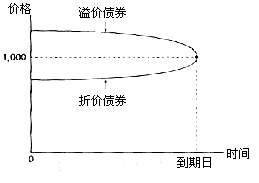
\includegraphics[width=0.3\textwidth]{1.png}

            \maketitle{定理三可以解释斜率绝对值增大}
        \end{center}
    \end{figure}
    零息票债券的价格变动有其特殊性。在到期日,债券价格等于面值,到期日之前,由于资金的时间价值,债券价格低于面值,并且随着到期日的临近而趋近于面值。如果利率恒定,则价格以等于利率值的速度上升。
    \item 息票率\\
    息票率决定了未来现金流的大小。在其他属性不变的条件下,债券的息票率越低,
    债券价格随预期收益率波动的幅度越大。(本金占的比例更大)
    \item 可赎回条款:在一定时间内发行人有权赎回债券\\
    赎回价格:初始赎回价格通常设定为债券面值加上年利息,并且随着到期时间的减少而下降,逐渐趋近于面值。
    赎回价格的存在制约了债券市场价格的上升空间,并且增加了投资者的交易成本,所以,降低了投资者的投资收益率。

    赎回保护期:在保护期内,发行人不得行使赎回权,一般是发行后的5至10年。

    可赎回条款对债券收益率影响:
    可赎回条款的存在,降低了该类债券的内在价值,并且降低了投资者的实际收益率。
    息票率越高,发行人行使赎回权的概率越大,即投资债券的实际收益率与债券承诺的收益率之间的差额越大。为弥补被赎回的风险,
    这种债券发行时通常有较高的息票率和较高的承诺到期收益率。在这种情况下,投资者关注赎回收益率(YTC),而不是到期收益率(YTM)。

    赎回收益率:赎回收益率也称为首次赎回收益率(YTC),它假设公司一旦有权利就执行可赎回条款。

    折价发行:如果债券折价较多,价格远低于赎回价格,即使市场利率下降也不会高于赎回价格,公司就不会赎回债券,
    也即折价债券提供了隐性赎回保护。对折价债券主要关注到期收益率。

    溢价发行:溢价债券由于发行价较高,极易被赎回。所以,对溢价债券投资者主要关注赎回收益率。
    \item 税收待遇:税收待遇是影响债券的市场价格和收益率的一个重要因素
    \item 流通性:指债券投资者将手中的债券变现的能力\\
    通常用债券的买卖差价的大小反映债券的流动性大小。买卖差价较小的债券流动性比较高;反之,流动性较低。

    在其他条件不变的情况下,债券的流动性与债券的名义到期收益率之间呈反比例关系;债券的流动性与债券的内在价值呈正比例关系。
    \item 违规风险:债券发行人未履行契约规定支付的债券本金和利息,给债券投资者带来损失的可能性\\
    债券评级是反映债券违约风险的重要指标,债券评级的主要财务比率:
    \begin{enumerate}
        \item 固定成本倍数:即公司收益与固定成本之比
        \item 杠杆比率:即资产负债比率 
        \item 流动性比率:流动比率和速动比率
        \item 盈利性比率:常见的是资产收益率
        \item 现金比率,即公司现金与负债之比
        \item 奥尔特曼的分离分析
    \end{enumerate}
    \item 可转换性:可转换债券的持有者可用债券来交换一定数量的普通股股票。\\
    转换率:每单位债券可换得的股票股数 
    
    市场转换价值:可换得的股票当前价值

    转换损益:债券价格与市场转换价值的差额

    可转换债券息票率和承诺的到期收益率通常较低。
    但是,如果从转换中获利,则持有者的实际收益率会大于承诺的收益率。

    \item 可延期性\\
    \textbf{与可赎回债券相比},它给予持有者而不是发行者一种终止或继续拥有债券的权利。

    如果市场利率低于息票率,投资者将继续拥有债券;
    反之,如果市场利率上升,超过了息票率,投资者将放弃这种债券,收回资金,投资于其他收益率更高的资产。
    这一规定有利于投资者,所以可延期债券的息票率和承诺的到期收益率\textbf{较低}。
\end{itemize}
\begin{figure}[H]
    \begin{center}
        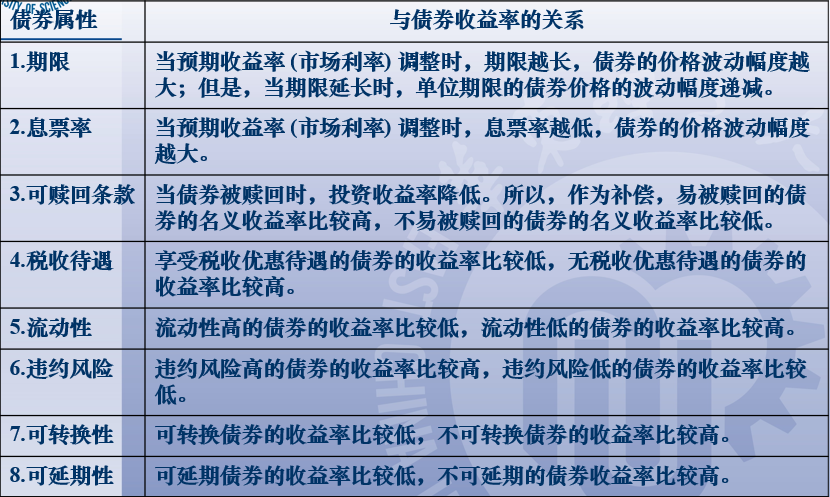
\includegraphics[width=1\textwidth]{2.png}
    \end{center}
\end{figure}
\clearpage

\subsection*{久期-债券持有者收回其全部本金和利息的平均时间}
马考勒久期:
\[D=\frac{\sum_{t=1}^{T}{\frac{c_t}{\left(1+y\right)^t}\times t}}{P}=\sum_{t=1}^{T}{[\frac{c_t/\left(1+y\right)^t}{P}}\times\ t]=\sum_{t=1}^{T}{[\frac{PV\left(c_t\right)}{P}}\times\ t]\]
\begin{enumerate}
    \item 只有贴现债券的马考勒久期等于它们的到期时间。
    \item 直接债券的马考勒久期小于或等于它们的到期时间。只有仅剩最后一期就要期满的直接债券的马考勒久期等于它们的到期时间,并等于1 。
    \item 统一公债的马考勒久期等于$1+\frac{1}{y}$,其中y是计算现值采用的贴现率。
    \item 在到期时间相同的条件下,息票率越高,久期越短。
    \item 在息票率不变的条件下,到期时间越长,久期一般也越长。
    \item 在其他条件不变的情况下,债券的到期收益率越低,久期越长。
\end{enumerate}

货币久期$(\$D=D\times P)$:利率变动引起的价值变动绝对金额。
\[D\times P=-\frac{\text{d}P}{\text{d}y}\]

修正久期(新的久期,久期):(如果使用连续复利来定价,就不存在马考勒久期和修正久期的区别了)
\[D^\ast=\frac{D}{1+y}\]

久期的缺陷:
现实生活中,债券价格变动率和收益率变动之间的关系并不是线性关系,而是非线性关系。
如果只用久期来估计收益率变动与价格变动率之间的关系,
收益率上升或下跌一个固定的幅度时,价格下跌或上升的幅度是一样的。显然这与事实不符。
\clearpage



\subsection*{凸度:债券价格变动率与收益率变动关系曲线的曲度}
\[C=\frac{1}{P}\frac{\partial^2P}{\partial y^2}\]
收益率下降时,价格的实际上升率高于用久期计算出来的近似值,而且凸度越大,实际上升率越高;
当收益率上升时,价格的实际下跌比率却小于用久期计算出来的近似值,且凸度越大,价格的实际下跌比率越小。
\begin{figure}[H]
    \begin{center}
        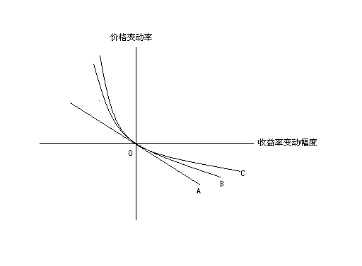
\includegraphics[width=0.5\textwidth]{3.png}

        \maketitle{A:久期 ;B,C:凸度}
    \end{center}
\end{figure}
\begin{enumerate}
    \item 当收益率变动幅度较大时,用久期近似计算的价格变动率就不准确,需要考虑凸度调整
    \item 在其他条件相同时,人们应该偏好凸度大的债券
\end{enumerate}
当收益率变动幅度不太大时,收益率变动幅度与价格变动率之间的关系就可以近似表示为:(价格变动=久期+凸度)
\[\frac{\Delta P}{P}=-D^*\Delta y+\frac{1}{2}C(\Delta y)^2\]

\subsection*{免疫-两种作用相互抵消的利率风险:价格风险和再投资风险}
久期免疫:如果资产组合的久期选择得当,这一资产组合的久期恰好与投资者的持有期相等时,
价格风险与再投资风险将完全抵消,到期时投资组合的累积价值将不受利率波动的影响。

免疫资产的构造:先计算实现承诺的现金流出的久期,然后投资于一组具有相同久期的债券资产组合。

本质:无论利率如何变动,资产与负债的久期匹配可以确保资产组合有偿还负债的能力。

久期免疫的缺陷:久期是对债券价格变化的一阶近似,因此,一般来说,久期会低估利率变动带来的预期收益或损失。

改进方法:由于凸度是二阶估计,考虑凸度可以提高利用久期得到的结果 ,尤其是在利率变化很大时,凸度可以修正通过久期得到关于债券价格变化的估计

\clearpage
\section*{\center 债券价值分析重要概念}
\begin{tcolorbox}
    \begin{itemize}
        \item 收入资本化法:任何资产的内在价值均取决于该资产预期的未来现金流的现值
        \item 贴现债券:零息债券,以低于面值发行,不支付利息,到期按债券面值偿还的债券
        \item 直接债券:定息债券或固定利息债券,按照票面金额计算利息,票面上可附有作为定期支付利息凭证的息票,也可不附息票。
        \item 统一公债:没有到期日的特殊的定息债券
        \item 息票率:年利息收入与债券面额之比率,决定了未来现金流的大小。
        \item 可赎回条款:在一定时间内发行人有权赎回债券。
        \item 可赎回收益率:假设公司一旦有权力就执行可赎回条款
        \item 流通性:指债券投资者将手中的债券变现的能力
        \item 违约风险:债券发行人未履行契约规定支付的债券本金和利息,给债券投资者带来损失的可能性。
        \item 信用评级:以分析发行者财务指标的水平及趋势为基础,对其债券质量做出分类评定
        \item 可转换性:可转换债券的持有者可用债券来交换一定数量的普通股股票
        \item 可延期性:给予持有者而不是发行者一种终止或继续拥有债券的权力。
        \item 债券定价原理:马尔基尔提出的5个原理
        \item 马考勒久期:使用加权平均数的形式计算债券的平均到期时间。只是久期计算公式的一部分,并非真正的久期
        \item 修正的久期:对于给定的到期收益率的微小变动,债券价格的相对变动与其麦考利久期的比例。
        \item 久期:债券各期现金流支付所需时间的加权平均值
        \item 货币久期:利率变动引起的价值变动的绝对金额
        \item 凸度:债券价格变动率与收益率变动关系曲线的曲度
        \item 免疫:投资者或金融机构用来保护他们的全部金融资产免受利率波动影响的策略
    \end{itemize}
\end{tcolorbox}


\end{document}